\chapter{Bazel}
\section{Bazel start}
\subsection{用工作空间}
所有的构建发生在一个存在于你的文件系统并且包含你想构建软件的源代码的目录workspace中,正如build输出的符号连接的目录(例如bazel-bin和bazel-out),构建发生在workspace。workspace的位置目录不重要,但是必须包含一个叫做WORKSPACE的顶层目录;一个空文件是一个可用的workspace。WORKSPACE文件能被用来查询构建输出需要的外部依赖。一个workspace可以在多个项目中共享。
\begin{lstlisting}[language=Bash]
touch WORKSPACE
\end{lstlisting}
\subsection{创建一个构建文件}
为了知道你的工程中什么目标能被构建,Bazel查看BUILD文件。它的语法类似Python被写进Bazel的构建语言中。通常它们仅仅是一个声明规则的序列。每个规则指定它的输入,输出和一个从输入到输出的计算方法。

规则对于那些已经在\href{https://docs.bazel.build/versions/master/be/general.html#genrule}{genrule}前用过Makefile的人来说通常很熟悉,可以通过shell命令指定如何生成输出。
\begin{lstlisting}[language=Bash]
genrule(
  name = ``hello'',
  outs = [``hello_world.txt''],
  cmd = ``echo Hello World > $@",
      )
\end{lstlisting}
shell命令包含\href{https://docs.bazel.build/versions/master/be/make-variables.html}{make变量}
用上面的BUILD文件你可以要求Bazel生成目标
\begin{lstlisting}[language=Bash]
\end{lstlisting}
\begin{lstlisting}[language=Bash]
$ bazel build :hello
.
INFO: Found 1 target...
Target //:hello up-to-date:
  bazel-genfiles/hello_world.txt
  INFO: Elapsed time: 2.255s, Critical Path: 0.07s
\end{lstlisting}
我们注意到两件事,第一:目标通常通过它们的\href{https://docs.bazel.build/versions/master/build-ref.html#labels}{label}访问label规则的\href{https://docs.bazel.build/versions/master/be/general.html#genrule.name}{name}属性指定,第二:Bazel将生成的文件放进一个分割的目录(bazel-genfiles目录通常是符号链接)只要不污染你的源树。

规则用其它规则的输出作为输入,下面的例子,再一次生成的源代码被它们的label访问:
\begin{lstlisting}[language=Bash]
genrule(
  name = ``hello'',
  outs = [``hello_world.txt''],
  cmd = ``echo Hello World > $@",
)
genrule(
  name = "double",
  srcs = [":hello"],
  outs = ["double_hello.txt"],
  cmd = "cat $< $< > $@",
)
\end{lstlisting}
最后注意生成规则看着很类似,它不是最好的规则。它是为不同的语言指定规则的首选。
\subsection{下一步}
在Java和C++程序上构建。
\section{构建C++工程}
在这个导航中,你将学习通过Bazel构建C++应用的基础,你讲设置你的workspace建立一个简单的工程说明关键的Bazel概念,像target个BIULD文件,在完成这个导航后,查看\href{https://docs.bazel.build/versions/master/tutorial/cpp-use-cases.html}{Common C++ Build User Cases}了解更多像写,运行C++测试的高级概念。
\subsection{你将学习}
\begin{itemize}
	\item 构建目标
	\item 可视化项目依赖
	\item 分割项目成多个目标和包
	\item 在包上控制目标可视化
	\item 通过labels访问目标
\end{itemize}
\subsection{准备}
开始之前你需要确保安装合适的Bazel,然后访问Bazel的GitHub仓库获取示例工程:
\begin{lstlisting}[language=Bash]
git clone https://github.com/bazelbuild/examples/
\end{lstlisting}
示例工程的examples/cpp-tutorial目录结构如下:
\begin{figure}[H]
	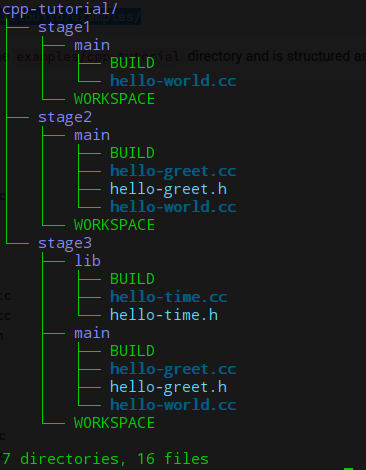
\includegraphics[scale=0.5]{cpp-tutorial.png}
\end{figure}
如你所见导航中有一些文件,每个集合代表一个stage,你将构建一个单独的目标到单独的包,第二个stage你讲分割你的工程为多个目标但是保持在一个单独的包中。在第三个和最后的stage,你讲分割你的工程为多个package并且用不同的targets构建它。
\subsection{构建Bazel}
\subsubsection{建立你的workspace}
在你可以构建你的工程之前,你需要建立你的workspace。一个workspace是一个保存你工程的源代码文件和Bazel的构建输出的目录。它也包含Bazel识别为特殊文件的文件:
\begin{itemize}
	\item WORKSPACE文件识别一个目录和它的内容作为一个Bazel workspace同时生成工程的根目录结构。
	\item 一个或者更多的BUILD文件告诉Bazel如何构建工程的不同部分。(在workspace的一个目录包含BUILD文件是一个包。你将在之后的导航中学习包)
\end{itemize}
为了设计一个目录作为Bazel workspace,在目录中创建一个空的名字为WORKSPACE的文件,当Bazel构建工程的时候,所有的输入和依赖必须在同一个workspace。文件保留在不同的workspace是是独立于其它的文件的除非被链接。
\subsection{明白BUILD文件}
一个BUILD文件包含一些针对Bazel的不同类型的指令。最重要的类型是build rule,它告诉Bazel如何构建想要的输出,像执行二进制或者库。在BUILD文件中的构建规则的实例称为target,指定一个指定的源代码文件西河和依赖。一个target也支出其它的目标。

查看在cpp-tutorial/stage1/main目录中BUILD文件
\begin{lstlisting}{language=Bash}
cc_binary(
    name = "hello-world",
    srcs = ["hello-world.cc"],
)
\end{lstlisting}
在我们的例子中,hello-world目标实例Bazel的內建\href{https://docs.bazel.build/versions/master/be/c-cpp.html#cc_binary}{cc\_binary rule}。规则告诉Bazel从hello-world.cc源文件的构建一个没有任何依赖自我包含执行二进制。
目标中的属性明确了它的依赖和选项状态。当name属性是命令,一些选项,例如hello-greet目标name是自我说明,srcs指定Bazel构建目标的源文件。
\subsection{构建工程}
让我们建立你的样本工程,进入cpp-tutorial/stage1目录运行下面的代码
\begin{lstlisting}[language=Bash]
bazel build //main:hello-world
\end{lstlisting}
注意目标label//main:部分是BUILD文件获取workspace根的位置,hello-world是我们在BUILD文件中命名目标的名字。

Bazel将产生类似下面的输出:
\begin{lstlisting}[language=Bash]
INFO: Found 1 target...
Target //main:hello-world up-to-date:
  bazel-bin/main/hello-world
  INFO: Elapsed time: 6.817s, Critical Path: 0.54s
\end{lstlisting}
恭喜你你已经构建了你的第一个Bazel目标!Bazel防止build输出在workspace的根目录的bazel-bin目录。通过它的内容得到Bazel的输出结构,现在测试你的构建库:
\begin{lstlisting}[language=Bash]
bazel-bin/main/hello-world
\end{lstlisting}
\subsection{回顾依赖图}
一个成功的构建在BUILD文件有一些明确状态的依赖。Bazel用这些状态创建工程的依赖图,是的增量构建更精确。让我们可视化我们样例工程依赖,首先生成一个依赖图的文字表示(在workspace根目录运行命令):
\begin{lstlisting}[language=Bash]
bazel query --nohost_deps --noimplicit_deps 'deps(//main:hello-world)' \
  --output graph
\end{lstlisting}
上面的命令告诉Bazel为目标//main:hello-world查找所有的依赖(包括多数依赖和隐藏依赖)输出为图表格式,然后粘贴文字到GraphViz。正如你所见,样例工程的第一个stage有一个目标没有额外依赖构建一个单个源文件:
\begin{figure}[H]
	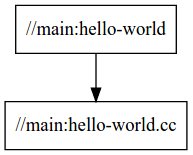
\includegraphics[scale=0.5]{dependency_graph.png}
\end{figure}
注意,你已经设置你的workspace,构建你的项目检查它的依赖,让我们增加一点复杂度。
\subsection{提炼你的Bazel构建}
尽管对于小的工程一个target是足够的,你也许将分割大的工程为多个目标包,运行快速的增量构建加速你的构建通过同时构建工程的多个部分。
\subsection{指定多个构建目标}
让我们分割我们的样本工程为两个目标,查看cpp-tutorial/stage2/main目录中的BUILD文件
\begin{lstlisting}[language=Bash]
cc_library(
    name = "hello-greet",
    srcs = ["hello-greet.cc"],
    hdrs = ["hello-greet.h"],
)
cc_binary(
    name = "hello-world",
    srcs = ["hello-world.cc"],
   deps = [
        ":hello-greet",
    ],
)
\end{lstlisting}
通过BUILD文件Bazel首先构建hello-greet库(用Bazel的內建\href{https://docs.bazel.build/versions/master/be/c-cpp.html#cc_library}{cc\_library rule}),然后hello-world二进制,在hello-world目标的deps属性告诉Bazel hello-greet库要求构建hello-world二进制。构建一个新版,进入cpp-tutorial/stage2目录运行下面的命令:
\begin{lstlisting}[language=Bash]
bazel build //main:hello-world
\end{lstlisting}
Bazel生成类似下面的输出:
\begin{lstlisting}[language=Python]
INFO: Found 1 target...
Target //main:hello-world up-to-date:
  bazel-bin/main/hello-world
  INFO: Elapsed time: 6.625s, Critical Path: 0.76s
\end{lstlisting}
现在测试你构建的二进制:
\begin{lstlisting}[language=Bash]
bazel-bin/main/hello-world
\end{lstlisting}
如果你修改hello-greet.cc,重新构建工程Bazel将仅仅重新编译这个文件,查看依赖图,你可以看到hello-world依赖和之前相同的输入,但是构建的结构有点不同:
\begin{figure}[h]
	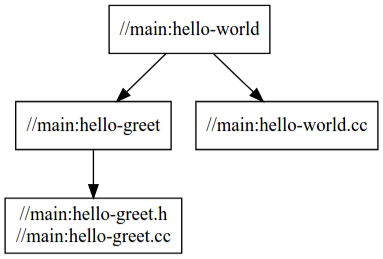
\includegraphics[scale=0.5]{dependency_graph1.png}
\end{figure}
你也许构建两个目标,hello-world目标构建一个源文件依赖另一个其它的目标(//main:hello-greet),构建两个额外的源文件。
\subsection{用多个包}
让我们分割工程为多个包,查看cpp-tutorial/stage3目录:
\begin{center}
\begin{figure}[h]
	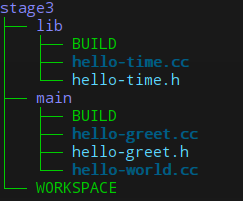
\includegraphics[scale=0.5]{mult_package}
\end{figure}
\end{center}
注意我们现在有两个子目录,每个包含一个BUILD文件,因此对于Bazel,workspace现在包含两个包lib和main.
查看lib/BUILD文件:
\begin{lstlisting}[language=Bash]
cc_library(
    name = "hello-time",
    srcs = ["hello-time.cc"],
    hdrs = ["hello-time.h"],
    visibility = ["//main:__pkg__"],
)
\end{lstlisting}
main/BUILD文件:
\begin{lstlisting}[language=Python]
cc_library(
    name = "hello-greet",
    srcs = ["hello-greet.cc"],
    hdrs = ["hello-greet.h"],
)
cc_binary(
    name = "hello-world",
    srcs = ["hello-world.cc"],
    deps = [
        ":hello-greet",
        "//lib:hello-time",
    ],
)
\end{lstlisting}
正如你看到的main包中的hello-world目标依赖lib中的于hello-time目标(因此目标标签//lib:hello-time)Bazel知道这通过deps属性。查看依赖图:
\begin{figure}[h]
	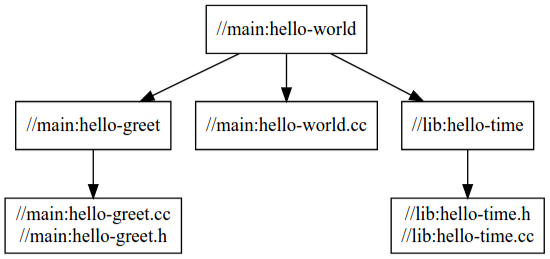
\includegraphics[scale=0.5]{dependency_graph2.png}
\end{figure}
注意对于成功的构建,我们在lib/BUILD创建一个//lib:hello-time目标在main/BUILD中用visibility属性明确的可视化目标。这是因为默认目标仅仅对在同一BUILD文件中的其它的目标可见。(Bazel用目标可视化阻止了包含实现细节泄露到公开的api的问题)
当我们构建我们工程的最终版本,进入cpp-tutorial/stage3目录运行下面的命令:
\begin{lstlisting}[language=Bash]
bazel build //main:hello-world
\end{lstlisting}
Bazel生成类似下面的输出:
\begin{lstlisting}[language=Bash]
INFO: Found 1 target...
Target //main:hello-world up-to-date:
  bazel-bin/main/hello-world
  INFO: Elapsed time: 6.584s, Critical Path: 0.76s
\end{lstlisting}
现在测试最新的构建二进制文件:
\begin{lstlisting}[language=Bash]
bazel-bin/main/hello-world
\end{lstlisting}
你现在将构建有两个包三个目标的工程明白它们之间的依赖。
\subsection{用标签访问目标}
在BUILD文件和在命令行,Bazel用labels访问目标,例如//main:hello-world或者lib//hello-time。它们的语法:
\begin{lstlisting}[language=Bash]
//path/to/package:target-name
\end{lstlisting}
如果目标是一个规则目标,然后path/to/package是一个包含BUILD文件的路径,target-name是你在BUILD文件中命名的名字。如果目标是一个规则目标然后path/to/package是package的根目录,target-name是目标文件的名字,包含完整的路径。当在同一个包中访问目标,你可以用//:target-name跳过包。
\subsection{进一步阅读}
恭喜你!你现在知道的用Bazel构建C++工程的基础,下一步,读更常用的\href{https://docs.bazel.build/versions/master/tutorial/cpp-use-cases.html}{C++ build use cases},然后检查下面:
\begin{itemize}
	\item \href{https://docs.bazel.build/versions/master/external.html}{External Dependencies}了解更多本地和远程仓库。
	\item \href{https://docs.bazel.build/versions/master/be/overview.html}{Build Encyclopedia}了解更多Bazel
	\item \href{https://docs.bazel.build/versions/master/tutorial/java.html}{Java build tutorial}开始用Bazel构建Java 程序
	\item \href{https://docs.bazel.build/versions/master/tutorial/app.html}{mobile application tutorial}开始用Bazel为Android和IOS构建移动程序。
\end{itemize}
\section{常用的C++构建情况}
\subsection{一个目标中有多个文件}
你可以用\href{https://docs.bazel.build/versions/master/be/functions.html#glob}{glob}包含多个文件,例如:
\begin{lstlisting}[language=Bash]
cc_library(
    name = "build-all-the-files",
    srcs = glob(["*.cc"])
    hdrs = glob(["*.h"]),
)
\end{lstlisting}
在这个目标中Bazel将构建所有在相同目录中找到的.cc和.h文件作为包含这个目标的BUILD文件
\subsection{用include}
如果一个文件包含一个头文件,然后文件的规则依赖于头文件的库。相关,仅仅直接以来需要制定为依赖。例如,假设sandwich.h包含bread.h同事bread.h包含flour.h。sandwith.h不包含flour.h(在他的sandwich中谁想要flour?)因此BUILD文件将看起来像这样:
\begin{lstlisting}[language=Bash]
cc_library(
    name = "sandwich",
    srcs = ["sandwich.cc"],
    hdrs = ["sandwich.h"],
    deps = [":bread"],
)
cc_library(
    name = "bread",
    srcs = ["bread.cc"],
    hdrs = ["bread.h"],
    deps = [":flour"],
)
cc_library(
    name = "flour",
    srcs = ["flour.cc"],
    hdrs = ["flour.h"],
)
\end{lstlisting}
这里sandwich库依赖于bread,bread依赖于flour库。
\subsection{添加包含路径}
有时候你不想根目录在workspace目录中包含,存在的库也许已经有一个包含目录,但是这个不露不和你的workspace路径匹配。例如,假设你有下面的文件结构:
\begin{lstlisting}[language=Bash]
└── my-project
    ├── third_party
    │   └── some_lib
    │       ├── BUILD
    │       ├── include
    │       │   └── some_lib.h
    │       └── some_lib.cc
    └── WORKSPACE
\end{lstlisting}
Bazel将希望same\_lib.h被包含作为third\_party/some\_lib/include/some\_lib.h,但是假设some\_lib.cc包含"include/some\_lib.h".为了包含路径可用。third\_party/some\_lib/BUILD将需要制定some\_lib/目录是一个包含目录:
\begin{lstlisting}[language=Bash]
cc_library(
    name = "some_lib",
    srcs = ["some_lib.cc"],
    hdrs = ["some_lib.h"],
    copts = ["-Ithird_party/some_lib"],
)
\end{lstlisting}
这对于外部依赖特别有用,尽管他们的头文件必须用一个/前缀包括。
\subsection{包含外部的库}
假设你用\href{https://github.com/google/googletest}{Google Test}。你可以在WORKSPACE文件用一个new\_仓库函数下载Google Test使得它是你的可用仓库:
\begin{lstlisting}[language=Bash]
new_http_archive(
    name = "gtest",
    url = "https://github.com/google/googletest/archive/release-1.7.0.zip",
    sha256 = "b58cb7547a28b2c718d1e38aee18a3659c9e3ff52440297e965f5edffe34b6d0",
    build_file = "gtest.BUILD",
)
\end{lstlisting}
\begin{quote}
	\emph{注意:如果目标已经包含一个BUILD文件,你可以用一个non-new\_函数}
\end{quote}
然后创建gtest.BUILD和BUILD文件编译Google Test。Google Test有一些特别的要求使得他的cc\_library规则更复杂:
\begin{itemize}
	\item googletest-release-1.7.0/src/gtest-all.cc \#includes 所有的在googletest-release-1.7.0/src/的文件,因此我们需要通过编译器执行它或者我们对于一样的符号将得到连接错误
	\item 它用和googletest-release-1.7.0/include/目录下的头文件("gtest/gtest.h"),因此我们必须添加这个目录到包含路径。
	\item 它需要连接进ptread,因此我们添加linkopt
\end{itemize}
完整的规则如下:
\begin{lstlisting}[language=Python]
cc_library(
    name = "main",
    srcs = glob(
    ["googletest-release-1.7.0/src/*.cc"],
     exclude = ["googletest-release-1.7.0/src/gtest-all.cc"]
    ),
     hdrs = glob([
        "googletest-release-1.7.0/include/**/*.h",
        "googletest-release-1.7.0/src/*.h"
    ]),
    copts = [
     "-Iexternal/gtest/googletest-release-1.7.0/include"
],
    linkopts = ["-pthread"],
    visibility = ["//visibility:public"],
)
\end{lstlisting}
这多少有些混乱:一切都是googletest-release-1.7.0的前缀作为一个归档结构的副产品。你可以创建new\_http\_archive通过添加strip\_prefix属性删除前缀:
\begin{lstlisting}[language=Bash]
new_http_archive(
    name = "gtest",
    url = "https://github.com/google/googletest/archive/release-1.7.0.zip",
    sha256 = "b58cb7547a28b2c718d1e38aee18a3659c9e3ff52440297e965f5edffe34b6d0",
    build_file = "gtest.BUILD",
    strip_prefix = "googletest-release-1.7.0",
)
\end{lstlisting}
然后gtest.BUILD看起来像这样:
\begin{lstlisting}[language=Bash]
cc_library(
    name = "main",
    srcs = glob(
     ["src/*.cc"],
      exclude = ["src/gtest-all.cc"]
    ),
     hdrs = glob([
	        "include/**/*.h",
	        "src/*.h"
	    ]),
    copts = ["-Iexternal/gtest/include"],
    linkopts = ["-pthread"],
    visibility = ["//visibility:public"],
)
\end{lstlisting}
现在cc\_规则可以依赖于\@gtest//:main
\subsection{写,运行一个C++ Test}
例如,我们可以创建一个测试像下面这样./test/hello-test.cc:
\begin{lstlisting}[language=Bash]
#include "gtest/gtest.h"
#include "lib/hello-greet.h"

TEST(HelloTest, GetGreet) {
  EXPECT_EQ(get_greet("Bazel"), "Hello Bazel");
}
\end{lstlisting}
然后为你的tests床键文件./test/BUILD文件:
\begin{lstlisting}[language=Bash]
cc_test(
    name = "hello-test",
    srcs = ["hello-test.cc"],
    copts = ["-Iexternal/gtest/include"],
    deps = [
        "@gtest//:main",
        "//lib:hello-greet",
    ],
)
\end{lstlisting}
注意为了使得hello-greet对于hello-test可见,我们必须添加"//test:\_\_pkh\_\_"可视化在./lib/BUILD下的属性。现在你可以运行test
\begin{lstlisting}[language=Bash]
bazel test test:hello-test
\end{language=Bash}
这产生下面的输出:
\begin{lstlisting}[language=Bash]
INFO: Found 1 test target...
Target //test:hello-test up-to-date:
  bazel-bin/test/hello-test
  INFO: Elapsed time: 4.497s, Critical Path: 2.53s
  //test:hello-test PASSED in 0.3s

  Executed 1 out of 1 tests: 1 test passes.
\end{lstlisting}
\subsection{为预编译库添加依赖}
如果你想用你有一个编译过的库(例如,头文件和.so文件)打包它进cc\_library规则:
\begin{lstlisting}[language=Bash]
cc_library(
    name = "mylib",
    srcs = ["mylib.so"],
    hdrs = ["mylib.h"],
)
\end{lstlisting}
用这种方法,在你的workspace中的其它的C++目标可能依赖这个规则。
